\documentclass{article}

\usepackage{amsmath}
\usepackage{tikz}
\usetikzlibrary{positioning,decorations.markings,calc}
\usepackage{amssymb}
\usepackage{xcolor}

\definecolor{mygray}{RGB}{50,49,51}
\definecolor{mygray2}{RGB}{70,70,70}
\definecolor{mywhite}{RGB}{197,192,195}
\definecolor{myblue}{RGB}{0, 161, 241}
\definecolor{myyellow}{RGB}{255, 187, 0}
\definecolor{mygreen}{RGB}{124, 187, 0}
\definecolor{myred}{RGB}{246, 83, 20}

\begin{document}
\begin{center}
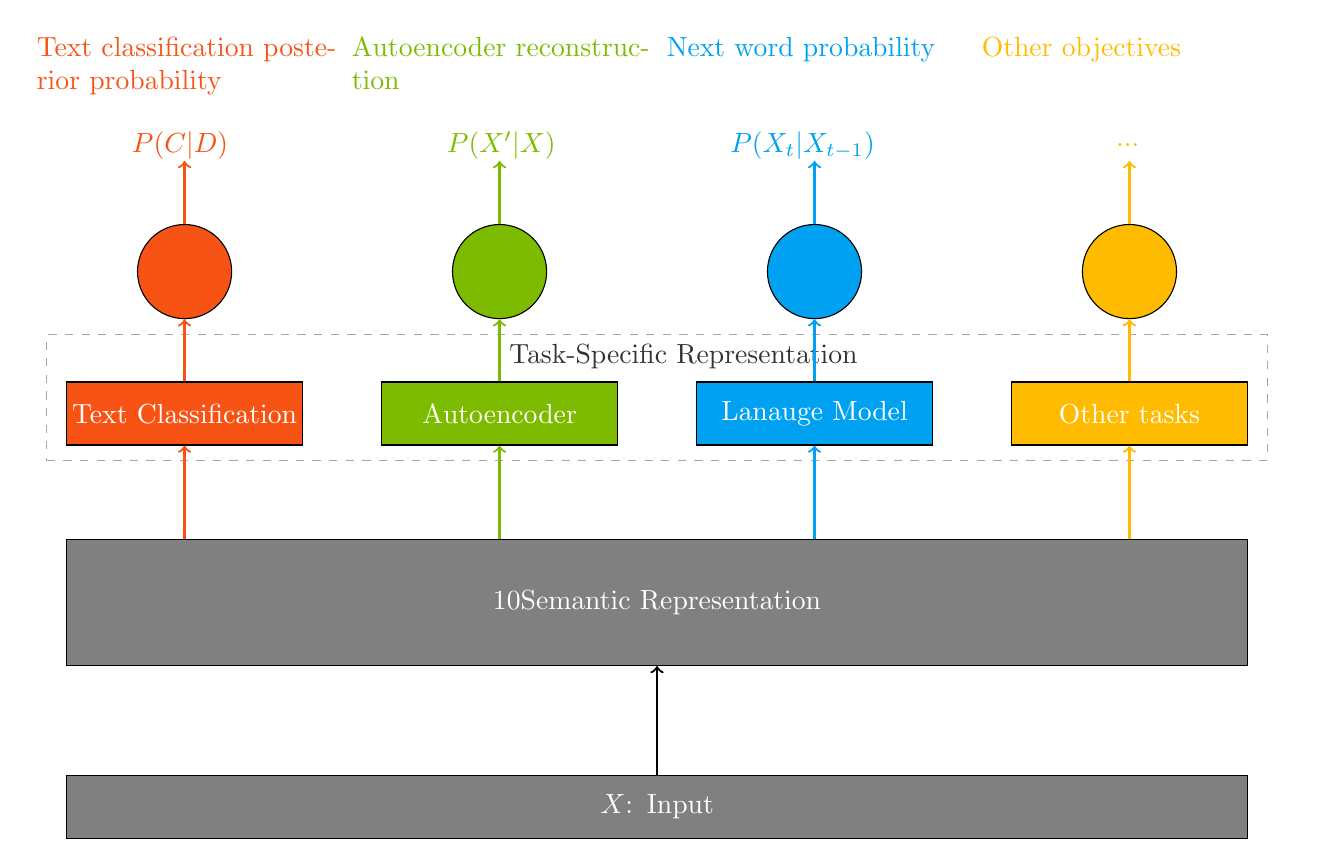
\begin{tikzpicture}[%
	%common options for blocks
	block/.style = {draw,fill=lightgray, align=center, anchor=west, minimum height=0.8cm, inner sep=0},
	largeblock/.style = {draw,fill=lightgray, align=center, anchor=west, minimum height=1.6cm, inner sep=0},
	dashblock/.style = {draw=gray,dashed,fill=lightgray, align=center, anchor=west, minimum height=1.6cm, inner sep=0},
	ball/.style = {circle, draw, align=center, anchor=north, inner sep=0, text width=1cm}%
]
   
\node[dashblock,anchor=north,text width=15.5cm,fill=white, opacity=0.7] (input) at (0,5.6) {};
\node[anchor=north west,text width=6cm, text=mygray] (tasknote) at (-2, 5.6){Task-Specific Representation};
   
\node[block,anchor=north,text width=15cm, fill=gray,text=white] (input) at (0,0) {$X$: Input};
\node[largeblock,anchor=north,text width=15cm, fill=gray, font=10, text=white] (rep) at (0,3) {Semantic Representation};

\node[block,anchor=north,text width=3cm, fill=myred, text=white] (tc) at (-6,5) {Text Classification};

\node[block,anchor=north,text width=3cm, fill=mygreen, text=white] (ae) at (-2,5) {Autoencoder};

\node[block,anchor=north,text width=3cm, fill=myblue, text=white] (lm) at (2,5) {Lanauge Model};

\node[block,anchor=north,text width=3cm, fill=myyellow, text=white] (ot) at (6,5) {Other tasks};

%\draw[thick,->,draw=black] (input.north) to (rep.south) node[anchor=east] at (0, 0.8) {$\mathbf{W_0}$};
\draw[thick,->,draw=black] (input.north) to (rep.south) node[anchor=east] at (0, 0.8) {};

\draw[thick,->,draw=myred] (-6, 3) to (tc.south) node[anchor=east] at (-6, 3.5) {};

\draw[thick,->,draw=mygreen] (-2, 3) to (ae.south) node[anchor=east] at (-2, 3.5) {};

\draw[thick,->,draw=myblue] (2, 3) to (lm.south) node[anchor=east] at (2, 3.5) {};

\draw[thick,->,draw=myyellow] (6, 3) to (ot.south) node[anchor=east] at (6, 3.5) {};


\node[ball, anchor=north,text width=1.2cm,fill=myred, text=white] (t1o) at (-6, 7) {};
\node[ball,anchor=north,text width=1.2cm,fill=mygreen, text=white] (t2o) at (-2,7) {};
\node[ball,anchor=north,text width=1.2cm,fill=myblue] (t3o) at (2,7) {};
\node[ball,anchor=north,text width=1.2cm,fill=myyellow] (t4o) at (6,7) {};

\draw[thick,->,draw=myred] (tc.north) to (t1o.south);
\draw[thick,->,draw=mygreen] (ae.north) to (t2o.south);
\draw[thick,->,draw=myblue] (lm.north) to (t3o.south);
\draw[thick,->,draw=myyellow] (ot.north) to (t4o.south);

\draw[thick,->,draw=myred,text=myred] (t1o.north) to (-6, 7.8) node[anchor=west] at (-6.8, 8) {$P(C|D)$};
\draw[thick,->,draw=mygreen,text=mygreen] (t2o.north) to (-2, 7.8) node[anchor=west] at (-2.8, 8) {$P(X'|X)$};

\draw[thick,->,draw=myblue,text=myblue] (t3o.north) to (2, 7.8) node[anchor=west] at (0.8, 8) {$P(X_{t}|X_{t-1})$};

\draw[thick,->,draw=myyellow,text=myyellow] (t4o.north) to (6, 7.8) node[anchor=west] at (5.7, 8) {$...$};


\node[anchor=north west,text width=4cm, text=myred] (cnote) at (-8, 9.5){Text classification posterior probability};

\node[anchor=north west,text width=4cm, text=mygreen] (cnote) at (-4, 9.5){Autoencoder reconstruction};

\node[anchor=north west,text width=4cm, text=myblue] (cnote) at (0, 9.5){Next word probability};

\node[anchor=north west,text width=4cm, text=myyellow] (cnote) at (4, 9.5){Other objectives};

\end{tikzpicture}
\end{center}
\end{document}